\documentclass[11pt,fleqn]{article}

\setlength {\topmargin} {-.15in}
\setlength {\textheight} {8.6in}

\usepackage{amsmath}
\usepackage{amssymb}
\usepackage{color}
\usepackage{tikz}
\usetikzlibrary{automata,positioning,arrows}
\usepackage{diagbox}
\usepackage{stackrel}

\newcommand{\be}{\begin{enumerate}}
\newcommand{\ee}{\end{enumerate}}

\begin{document}
\textbf{Exercise 4.4.33 Shortest Path in a grid:} Shortest path in a grid. Given an N-by-N matrix of positive integers, find the
shortest path from the $(0, 0)$ entry to the $(N-1, N-1)$ entry, where the length of the
path is the sum of the integers in the path. Repeat the problem but assume you can only
move right and down.\\

\textbf{Solution:} To find the shortest path, we can again use Dijkstra's Algorithm.

\begin{itemize}
	\item Step 1: We must first create an edge weighted Digraph by creating the possible adjacent edges to a cell in the grid. There can be a MAX of 4 edges adjacently connected to a cell> This consists of $UP,DOWN,LEFT,RIGHT$ nodes. However, there could still be less. For example, corners may only have 2 adjacent edges as the other 2 missing edges go outside the grid.
	
	\item We can do this by creating 2 arrays with 4 indices for representing each of the possible directions.
	
	\item 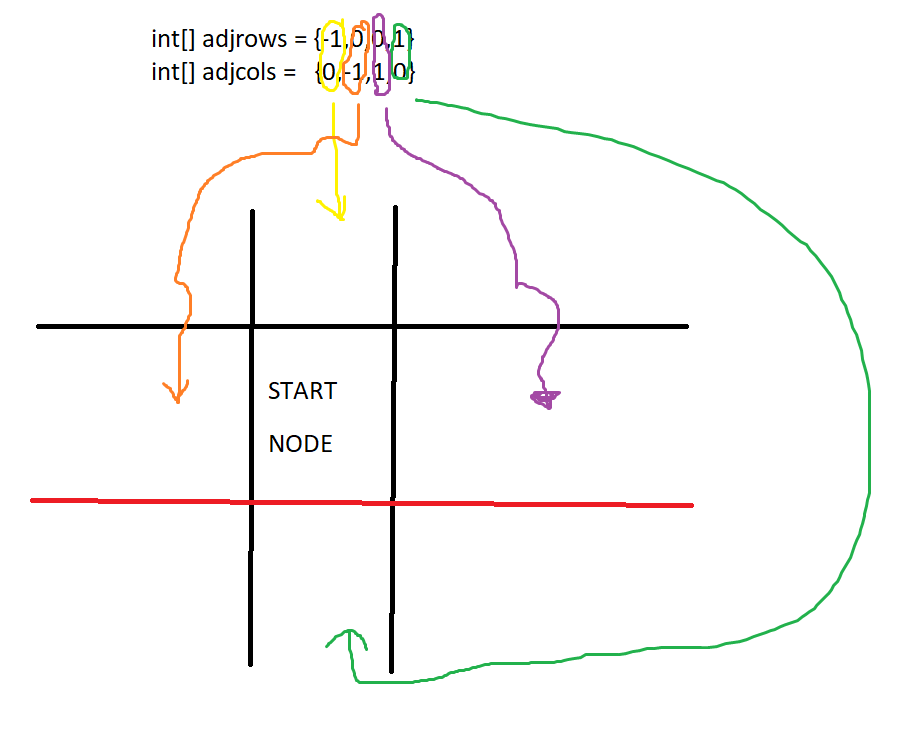
\includegraphics[scale=0.7]{4.4.33.png}
	
	\item For each cell in the matrix, we can iterate through adjrows and adjcols to create the edges and then check if they are valid cells prior to inserting into $edgeweightedDigraph$. Do this until reaches $(n-1,n-1)$ coordinate.
	
	\newpage
	
	\item Step 2: Once the $edgeweighteddigraph$ is complete, we can run Dijkstra's algorithm(code given on page 655 of textbook) where the length/weight of the edges will be the sum of the integers on the path of the grid.
\end{itemize}

For part b) of this problem, we can only move $right$ and $down$. The solution will be the exact same as before except the adjrows and adjcols arrays will be changed to only incorporate the coordinates for finding these points.\\

The arrays change to the following below.\\

$adjrows$ = {0,1}\\

$adjcols$ = {1,0}\\
\end{document}
